%%%%%%%%%%%%%%%%%%%%%%%%%%%%%%%%%%%%%%%%%
% Journal Article
% Distributed Parallel System
% Assignment 1
%
% Gahan M. Saraiya
% 18MCEC10
%
% References
% ==========
% https://computing.llnl.gov/tutorials/mpi/
% https://computing.llnl.gov/tutorials/mpi/#Routine_Arguments
%%%%%%%%%%%%%%%%%%%%%%%%%%%%%%%%%%%%%%%%%
\documentclass[11pt,a4paper,titlepage]{article}
\usepackage[a4paper]{geometry}
\usepackage[utf8]{inputenc}
\usepackage[english]{babel}
\usepackage{lipsum}
%\documentclass[12pt,letterpaper]{article}
%\usepackage{fullpage}
%\usepackage[top=2cm, bottom=4.5cm, left=2.5cm, right=2.5cm]{geometry}
%\usepackage{amsmath,amsthm,amsfonts,amssymb,amscd}
%\usepackage{lastpage}
%\usepackage{enumerate}
%\usepackage{fancyhdr}
%\usepackage{mathrsfs}
%\usepackage{xcolor}
%\usepackage{graphicx}
\usepackage{listings}
\usepackage{minted}
%\usepackage{hyperref}
%\usepackage{longtable}

\usepackage{amsmath, amssymb, amsfonts, amsthm, fouriernc, mathtools}
% mathtools for: Aboxed (put box on last equation in align envirenment)
\usepackage{microtype} %improves the spacing between words and letters

\usepackage{graphicx}
\graphicspath{ {./assets/} {./pics/} {./eps/}}
\usepackage{epsfig}
\usepackage{epstopdf}


%%%%%%%%%%%%%%%%%%%%%%%%%%%%%%%%%%%%%%%%%%%%%%%%%%
%% COLOR DEFINITIONS
%%%%%%%%%%%%%%%%%%%%%%%%%%%%%%%%%%%%%%%%%%%%%%%%%%
\usepackage[svgnames]{xcolor} % Enabling mixing colors and color's call by 'svgnames'
%%%%%%%%%%%%%%%%%%%%%%%%%%%%%%%%%%%%%%%%%%%%%%%%%%
\definecolor{MyColor1}{rgb}{0.2,0.4,0.6} %mix personal color
\newcommand{\textb}{\color{Black} \usefont{OT1}{lmss}{m}{n}}
\newcommand{\blue}{\color{MyColor1} \usefont{OT1}{lmss}{m}{n}}
\newcommand{\blueb}{\color{MyColor1} \usefont{OT1}{lmss}{b}{n}}
\newcommand{\red}{\color{LightCoral} \usefont{OT1}{lmss}{m}{n}}
\newcommand{\green}{\color{Turquoise} \usefont{OT1}{lmss}{m}{n}}
%%%%%%%%%%%%%%%%%%%%%%%%%%%%%%%%%%%%%%%%%%%%%%%%%%




%%%%%%%%%%%%%%%%%%%%%%%%%%%%%%%%%%%%%%%%%%%%%%%%%%
%% FONTS AND COLORS
%%%%%%%%%%%%%%%%%%%%%%%%%%%%%%%%%%%%%%%%%%%%%%%%%%
%    SECTIONS
%%%%%%%%%%%%%%%%%%%%%%%%%%%%%%%%%%%%%%%%%%%%%%%%%%
\usepackage{titlesec}
\usepackage{sectsty}
%%%%%%%%%%%%%%%%%%%%%%%%
%set section/subsections HEADINGS font and color
\sectionfont{\color{MyColor1}}  % sets colour of sections
\subsectionfont{\color{MyColor1}}  % sets colour of sections

%set section enumerator to arabic number (see footnotes markings alternatives)
\renewcommand\thesection{\arabic{section}.} %define sections numbering
\renewcommand\thesubsection{\thesection\arabic{subsection}} %subsec.num.

%define new section style
\newcommand{\mysection}{
    \titleformat{\section} [runin] {\usefont{OT1}{lmss}{b}{n}\color{MyColor1}} 
    {\thesection} {3pt} {} } 


%Importing csv as table
\usepackage{csvsimple}

\usepackage{longtable}
\renewcommand\thesection{\Roman{section}} % Roman numerals for the sections
\renewcommand\thesubsection{\Roman{subsection}} % Roman numerals for subsections
%----------------------------------------------------------------------------------------
%       DATE FORMAT
%----------------------------------------------------------------------------------------
\usepackage{datetime}
\newdateformat{monthyeardate}{\monthname[\THEMONTH], \THEYEAR}
%----------------------------------------------------------------------------------------

\titleformat{\section}[block]{\large\scshape\centering}{\thesection.}{1em}{} % Change the look of the section titles
\titleformat{\subsection}[block]{\large}{\thesubsection.}{1em}{} % Change the look of the section titles
\newcommand{\horrule}[1]{\rule{\linewidth}{#1}} % Create horizontal rule command with 1 argument of height
\usepackage{fancyhdr} % Headers and footers
\pagestyle{fancy} % All pages have headers and footers
\fancyhead{} % Blank out the default header
\fancyfoot{} % Blank out the default footer



%%%%%%%%%%%%%%%%%%%%%%%%%%%%%%%%%%%%%%%%%%%%%%%%%%
%		CAPTIONS
%%%%%%%%%%%%%%%%%%%%%%%%%%%%%%%%%%%%%%%%%%%%%%%%%%
\usepackage{caption}
\usepackage{subcaption}
%%%%%%%%%%%%%%%%%%%%%%%%
\captionsetup[figure]{labelfont={color=Turquoise}}

%%%%%%%%%%%%%%%%%%%%%%%%%%%%%%%%%%%%%%%%%%%%%%%%%%
%		!!!EQUATION (ARRAY) --> USING ALIGN INSTEAD
%%%%%%%%%%%%%%%%%%%%%%%%%%%%%%%%%%%%%%%%%%%%%%%%%%
%using amsmath package to redefine eq. numeration (1.1, 1.2, ...) 
%%%%%%%%%%%%%%%%%%%%%%%%
\renewcommand{\theequation}{\thesection\arabic{equation}}

%set box background to grey in align environment 
\usepackage{etoolbox}% http://ctan.org/pkg/etoolbox
\makeatletter
\patchcmd{\@Aboxed}{\boxed{#1#2}}{\colorbox{black!15}{$#1#2$}}{}{}%
\patchcmd{\@boxed}{\boxed{#1#2}}{\colorbox{black!15}{$#1#2$}}{}{}%
\makeatother
%%%%%%%%%%%%%%%%%%%%%%%%%%%%%%%%%%%%%%%%%%%%%%%%%%




%%%%%%%%%%%%%%%%%%%%%%%%%%%%%%%%%%%%%%%%%%%%%%%%%%
%% DESIGN CIRCUITS
%%%%%%%%%%%%%%%%%%%%%%%%%%%%%%%%%%%%%%%%%%%%%%%%%%
\usepackage[siunitx, american, smartlabels, cute inductors, europeanvoltages]{circuitikz}
%%%%%%%%%%%%%%%%%%%%%%%%%%%%%%%%%%%%%%%%%%%%%%%%%%



\makeatletter
\let\reftagform@=\tagform@
\def\tagform@#1{\maketag@@@{(\ignorespaces\textcolor{red}{#1}\unskip\@@italiccorr)}}
\renewcommand{\eqref}[1]{\textup{\reftagform@{\ref{#1}}}}
\makeatother
\usepackage{hyperref}
\hypersetup{colorlinks=true}

\usepackage{makecell}
\hypersetup{%
  colorlinks=true,
  linkcolor=blue,
  linkbordercolor={0 0 1}
}
 
\renewcommand\lstlistingname{Algorithm}
\renewcommand\lstlistlistingname{Algorithms}
\def\lstlistingautorefname{Alg.}

\lstdefinestyle{Python}{
    language        = Python,
    frame           = lines, 
    basicstyle      = \footnotesize,
    keywordstyle    = \color{blue},
    stringstyle     = \color{green},
    commentstyle    = \color{red}\ttfamily
}

\setlength{\parindent}{0.0in}
\setlength{\parskip}{0.05in}

%% Edit these as appropriate
%% \newcommand\course{CSE 3500}
%\newcommand\hwnumber{1}                  % <-- homework number
%\newcommand\NetIDa{Gahan M. Saraiya}           % <-- NetID of person #1
%\newcommand\NetIDb{18MCEC10}           % <-- NetID of person #2 (Comment this line out for problem sets)
%
%\pagestyle{fancyplain}
%\headheight 35pt
%\lhead{\NetIDa}
%\lhead{\NetIDa\\\NetIDb}                 % <-- Comment this line out for problem sets (make sure you are person #1)
%\chead{\textbf{\Large DPS Assignment \hwnumber}}
%\rhead{\course \\ \today}
%\lfoot{}
%\cfoot{}
%\rfoot{\small\thepage}
%\headsep 1.5em
%%%%%%%%%%%%%%%%%%%%%%%%%%%%%%%%%%%%%%%%%%%%%%%%%%
%% PREPARE TITLE
%%%%%%%%%%%%%%%%%%%%%%%%%%%%%%%%%%%%%%%%%%%%%%%%%%
\title{\blue Distributed Parallel System \\
    \blueb Assignment $1$}
\author{Gahan Saraiya (18MCEC10)}
%\date{\monthyeardate\today}
\date{March, 2019}
%%%%%%%%%%%%%%%%%%%%%%%%%%%%%%%%%%%%%%%%%%%%%%%%%%
%----------------------------------------------------------------------------------------
%       SET HEADER AND FOOTER
%----------------------------------------------------------------------------------------
\newcommand\theauthor{Gahan Saraiya}
\newcommand\thesubject{Distributed Parallel System}
\renewcommand{\footrulewidth}{0.4pt}% default is 0pt
\fancyhead[C]{Institute of Technology, Nirma University $\bullet$ \monthyeardate\today} % Custom header text
\fancyfoot[LE,LO]{\thesubject}
\fancyfoot[RO,LE]{Page \thepage} % Custom footer text
%----------------------------------------------------------------------------------------

\usepackage[utf8]{inputenc}
\usepackage[english]{babel}
\usepackage[utf8]{inputenc}
\usepackage{fourier} 
\usepackage{array}
\usepackage{makecell}

\renewcommand\theadalign{bc}
\renewcommand\theadfont{\bfseries}
\renewcommand\theadgape{\Gape[4pt]}
\renewcommand\cellgape{\Gape[4pt]}
\newcommand*\tick{\item[\Checkmark]}
\newcommand*\arrow{\item[$\Rightarrow$]}
\newcommand*\fail{\item[\XSolidBrush]}
\usepackage{minted} % for highlighting code sytax
\definecolor{LightGray}{gray}{0.9}
\renewcommand*{\arraystretch}{2}
%\definecolor{LightGray}{gray}{0.9}

\setminted[text]{
	frame=lines, 
	breaklines,
	baselinestretch=1.2,
	bgcolor=LightGray,
%	fontsize=\small
}
\setminted[bash]{
%	frame=lines, 
	breaklines,
	baselinestretch=1.2,
	bgcolor=LightGray,
%	fontsize=\small
}
\setminted[c]{
	frame=lines, 
	breaklines, 
	linenos,
	baselinestretch=1.2,
%	bgcolor=LightGray,
%	fontsize=\small
}


\begin{document}
\maketitle

\section{Write major MPI routine with its application, where to write (i.e.master/slave/any sender processor/any or all receiver) it's syntax and sample mpi statement with description. Use table to describe it and also mention Communication cost}

\begin{table}[!htbp]
    % \centering
    \hspace{-1cm}
    \begin{tabular}{l | p{4.5cm} | p{8cm}}
         \textbf{Routine} &  \textbf{Syntax} & \textbf{Description} \\ \hline
         \hline
             MPI\_Init 
             &  MPI\_Init (\&argc,\&argv) 
             & Initializes the MPI execution environment. This function must be called in every MPI program, before any other MPI functions and must be called only once in an MPI program.
         \\ \hline
            MPI\_Comm\_Size
            & MPI\_Comm\_size (comm,size)
            & Returns the total number of MPI processes in the specified communicator, such as MPI\_COMM\_WORLD. If the communicator is MPI\_COMM\_WORLD, then it represents the number of MPI tasks available to your application.
        \\ \hline
            MPI\_Comm\_rank
            & MPI\_Comm\_rank (comm,\&rank) 
            & Returns the rank of the calling MPI process within the specified communicator. Initially, each process will be assigned a unique integer rank between 0 and number of tasks - 1 within the communicator MPI\_COMM\_WORLD. 
            % This rank is often referred to as a task ID. If a process becomes associated with other communicators, it will have a unique rank within each of these as well.
        \\ \hline
            MPI\_Get\_processor\_name
            & MPI\_Get\_processor\_name (\&name,\&resultlength)
            & Returns the processor name. Also returns the length of the name. The buffer for "name" must be at least MPI\_MAX\_PROCESSOR\_NAME characters in size.
        \\ \hline
            MPI\_Wtime
            & MPI\_Wtime()
            & Returns an elapsed wall clock time in seconds (double precision) on the calling processor.
        \\ \hline
            MPI\_Finalize
            & MPI\_Finalize()
            & Terminates the MPI execution environment.
    \end{tabular}
    \caption{Environment Management Routines}
    \label{tab:EnvironmentManagementRoutines}
\end{table}

\subsection*{Example of Environment Management Routines}
\begin{minted}{c}
// required MPI include file  
#include "mpi.h"
#include <stdio.h>

int main(int argc, char *argv[]) {
int  numtasks, rank, len, rc; 
char hostname[MPI_MAX_PROCESSOR_NAME];

// initialize MPI  
MPI_Init(&argc,&argv);

// get number of tasks 
MPI_Comm_size(MPI_COMM_WORLD,&numtasks);

// get my rank  
MPI_Comm_rank(MPI_COMM_WORLD,&rank);

// this one is obvious  
MPI_Get_processor_name(hostname, &len);
printf ("Number of tasks= %d My rank= %d Running on %s\n", numtasks,rank,hostname);
// do some work with message passing 
// done with MPI  
MPI_Finalize();
}
\end{minted}

\subsection{Point to Point Communication Routines}
This point to point communication routines can be called by any node however if one node calls \verb|MPI_Send| routine then some other node in network must be calling \verb|MPI_Recv|. 

Hence to use this routine at least one sender is required and there should be one receiver to receive the data message.

\begin{table}[!htbp]
    % \centering
    \hspace{-2cm}
    \begin{tabular}{l | p{5cm} | p{5cm} | p{5cm}}
         \textbf{Routine} &  \textbf{Syntax} & \textbf{Description} & \textbf{Communication Cost}
         \\ \hline
         \hline 
            MPI\_Send
            & \makecell[tl]{
            MPI\_Send(
                \\ void* data, 
                \\ int count, 
                \\ MPI\_Datatype datatype, 
                \\ int destination, 
                \\ int tag, 
                \\ MPI\_Comm communicator
                \\ )
            }
            & almost every MPI call uses similar syntax. The first argument is the data buffer. The second and third arguments describe the count and type of elements that reside in the buffer. MPI\_Send sends the exact count of elements, and MPI\_Recv will receive at most the count of elements (more on this in the next lesson).
            & $ no\_of\_processor \times (Time_{startup} + Time_{data}) $
        \\ \hline
            MPI\_Recv
            & \makecell[tl]{
            MPI\_Recv(
                \\ void* data,
                \\ int count,
                \\ MPI\_Datatype datatype,
                \\ int source,
                \\ int tag,
                \\ MPI\_Comm communicator,
                \\ MPI\_Status* status)
            }
        & The fourth and fifth arguments specify the rank of the sending/receiving process and the tag of the message. The sixth argument specifies the communicator and the last argument (for MPI\_Recv only) provides information about the received message.
        & $ Time_{startup} + Time_{data} $
        \\ \hline
    \end{tabular}
    \caption{Point to Point Communication Routines}
    \label{tab:P2PCommunicationRoutines}
\end{table}

\subsection*{Example of Point to Point Communication}

\begin{minted}{c}
// Find out rank, size
int world_rank;
MPI_Comm_rank(MPI_COMM_WORLD, &world_rank);
int world_size;
MPI_Comm_size(MPI_COMM_WORLD, &world_size);

int number;
if (world_rank == 0) {
    number = -1;
    MPI_Send(&number, 1, MPI_INT, 1, 0, MPI_COMM_WORLD);
} else if (world_rank == 1) {
    MPI_Recv(&number, 1, MPI_INT, 0, 0, MPI_COMM_WORLD,
             MPI_STATUS_IGNORE);
    printf("Process 1 received number %d from process 0\n",
           number);
}
\end{minted}


\subsection{Collective Communication Routines}
These MPI routines are needs to be written at every node. Note that any node can invoke these routines.
\begin{table}[h]
    % \centering
    \hspace{-2cm}
    \begin{tabular}{l | p{5.5cm} | p{5cm} | p{4cm}}
         \textbf{Routine} &  \textbf{Syntax} & \textbf{Description} & \textbf{Communication Cost}
         \\ \hline
         \hline 
            MPI\_Bcast
            & \makecell[tl]{
            MPI\_Bcast(
                \\ void* data,
                \\ int count,
                \\ MPI\_Datatype datatype,
                \\ int root,
                \\ MPI\_Comm communicator)
            }
            & Broadcasts (sends) a message from the process with rank "root" to all other processes in the group
            & $ Time_{startup} + (no\_of\_processor \times Time_{data}) $
        \\ \hline
            MPI\_Scatter
            & \makecell[tl]{
                MPI\_Scatter(
                    \\ void* send\_data,
                    \\ int send\_count,
                    \\ MPI\_Datatype send\_datatype,
                    \\ void* recv\_data,
                    \\ int recv\_count,
                    \\ MPI\_Datatype recv\_datatype,
                    \\ int root,
                    \\ MPI\_Comm communicator
                )
            }
            & MPI\_Scatter is a collective routine that is very similar to MPI\_Bcast
            & $ Time_{startup} + (no\_of\_processor \times Time_{data}) $
        \\ \hline
            MPI\_Gather
            & \makecell[tl]{
            MPI\_Gather(
                \\ void* send\_data,
                \\ int send\_count,
                \\ MPI\_Datatype send\_datatype,
                \\ void* recv\_data,
                \\ int recv\_count,
                \\ MPI\_Datatype recv\_datatype,
                \\ int root,
                \\ MPI\_Comm communicator)
            }
            & Gathers distinct messages from each task in the group to a single destination task. This routine is the reverse operation of MPI\_Scatter
            & $ Time_{startup} + Time_{data} $
        \\ \hline
            MPI\_Reduce
            & \makecell[tl]{
                MPI\_Reduce(
                    \\ void* send\_data,
                    \\ void* recv\_data,
                    \\ int count,
                    \\ MPI\_Datatype datatype,
                    \\ MPI\_Op op,
                    \\ int root,
                    \\ MPI\_Comm communicator
                )
            }
            & Similar to MPI\_Gather, MPI\_Reduce takes an array of input elements on each process and returns an array of output elements to the root process. The output elements contain the reduced result.
            & $ Time_{startup} + Time_{data} $
    \end{tabular}
    \caption{Collective Communication Routines}
    \label{tab:CollectiveCommunicationRoutines}
\end{table}


\subsubsection*{Example of MPI\_Bcast}
\begin{minted}{c}
for (i = 0; i < num_trials; i++) {
    // Time my_bcast
    // Synchronize before starting timing
    MPI_Barrier(MPI_COMM_WORLD);
    total_my_bcast_time -= MPI_Wtime();
    my_bcast(data, num_elements, MPI_INT, 0, MPI_COMM_WORLD);
    // Synchronize again before obtaining final time
    MPI_Barrier(MPI_COMM_WORLD);
    total_my_bcast_time += MPI_Wtime();
    
    // Time MPI_Bcast
    MPI_Barrier(MPI_COMM_WORLD);
    total_mpi_bcast_time -= MPI_Wtime();
    MPI_Bcast(data, num_elements, MPI_INT, 0, MPI_COMM_WORLD);
    MPI_Barrier(MPI_COMM_WORLD);
    total_mpi_bcast_time += MPI_Wtime();
}
\end{minted}

\subsubsection*{Example of MPI\_Reduce}
\begin{minted}{c}
float *rand_nums = NULL;
rand_nums = create_rand_nums(num_elements_per_proc);

// Sum the numbers locally
float local_sum = 0;
int i;
for (i = 0; i < num_elements_per_proc; i++) {
  local_sum += rand_nums[i];
}

// Print the random numbers on each process
printf("Local sum for process %d - %f, avg = %f\n",
       world_rank, local_sum, local_sum / num_elements_per_proc);

// Reduce all of the local sums into the global sum
float global_sum;
MPI_Reduce(&local_sum, &global_sum, 1, MPI_FLOAT, MPI_SUM, 0,
           MPI_COMM_WORLD);

// Print the result
if (world_rank == 0) {
  printf("Total sum = %f, avg = %f\n", global_sum,
         global_sum / (world_size * num_elements_per_proc));
}

\end{minted}
In the code above, each process creates random numbers and makes a local\_sum calculation. The local\_sum is then reduced to the root process using MPI\_SUM. The global average is then $ global\_sum / (world\_size * num\_elements\_per\_proc) $

\section{Code for making ring, pass token from masters to others (ring topology)}
\inputminted{c}{src/3.ring.c}

\subsection*{Output}
\inputminted{text}{src/output_ring.txt}

% \inputminted[firstline=0,lastline=3]{text}{src/output_ring.txt}
\section{If no of processors $  < $ no of data given:
    {\footnotesize \\no of processors$  =5 $
    \\no of data $ =20 $
    \\pipeline constraints $ = $ until $ 4 $ data, then only all data will be forwarded to next processor.
    \\firstly, Complete till all processors then pass in bunch of four.}}
\begin{figure}[!htbp]
    \centering
    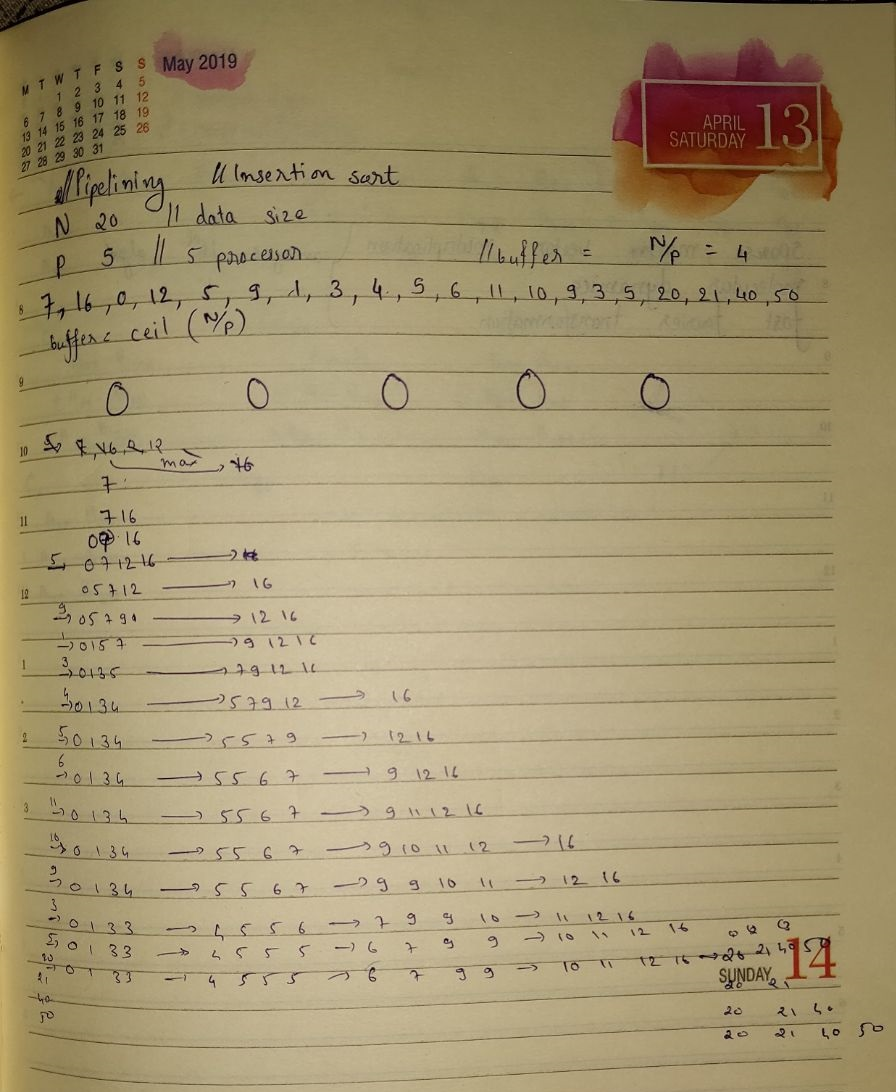
\includegraphics[width=0.9\textwidth]{pipeline}
\end{figure}
\section{Dwarfs of computing}
\begin{itemize}
    \item Dense linear algebra
    \item Sparse linear algebra
    \item Spectral methods
    \item N-body methods
    \item Structured grids
    \item Unstructured grids
    \item Monte Carlo methods
    \item MapReduce
    \item Combinational Logic
    \item Dynamic Programming
    \item Graph Traversal
    \item BackTracking and Branch and Bound
    \item Graphical Models
    \item Finite State Machine
\end{itemize}

\subsection{Dense linear algebra}
Problems can be Categorized based on scaling of operations vs. data volume as below:
\begin{itemize}
    \item BLAS level 1 ($ O(n) $)
        \\ Dot product, scale, copy, \dots
    \item BLAS level 2 ($ O(n^2) $)
        \\ $ Matrix \times Vector $, convolution, \dots
    \item BLAS level 3 ($ O(n^3) $)
        \\ $ Matrix \times Matrix $, dense eigenvalue solvers, matrix inversion, \dots
\end{itemize}

Existing implementations and libraries
\begin{itemize}
    \item BLAS, LAPACK
        \begin{itemize}
            \item Naïve implementations on netlib.org
            \item Vendor-optimized, shared-memory parallel implementations available (e.g., MKL, CUDABlas)
        \end{itemize}
    \item SCALAPACK
        \begin{itemize}
            \item Distributed-memory parallel LAPACK (netlib.org)
            \item Available, e.g., in Cluster MKL
        \end{itemize}
\end{itemize}

\subsection{Sparse linear Algebra}
“\verb|Sparse|”: $ N \times N $ Matrices have $ O(N) $ nonzero entries

\paragraph{Typical operation:} Sparse $ Matrix \times Vector $

Used in sparse eigenvalue solvers and solvers for systems of linear equations
\begin{itemize}
    \item Store only $ N_{nz} $ nonzero elements of matrix and RHS, LHS vectors
    \item with $ N_r $ (number of matrix rows) entries
    \item “Sparse”: $ N_{nz} ~ N_r $
    \item Type $ O(N)/O(N) \implies \text{memory bound} $ \footnote{Nevertheless, there is more than one loop here!}
\end{itemize}

\begin{figure}[!htbp]
    \centering
    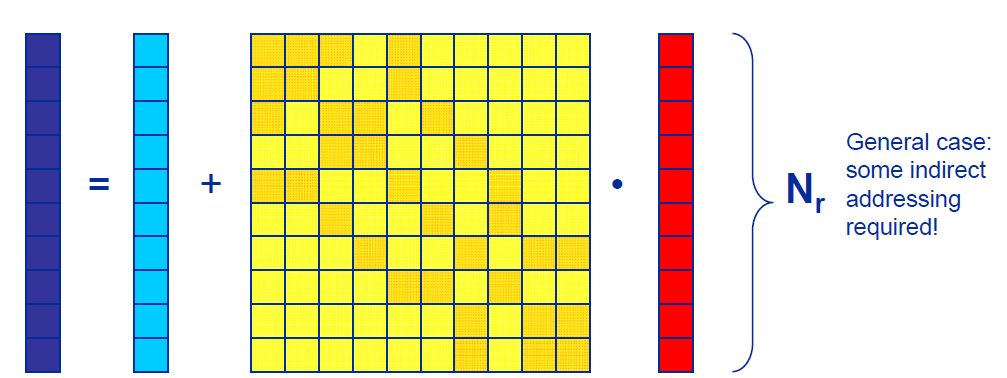
\includegraphics[width=0.7\textwidth]{sMvM}
    \caption{Sparse matrix-vector multiply (sMVM)}
\end{figure}

\subsection{Spectral methods}
\begin{itemize}
    \item $ O(N log N)/O(N) $
    \item Standard high performance implementation: FFTW
    \item MKL: Shared-memory parallel versions
    \item GPU: CUFFT
\end{itemize}
\begin{figure}[!htbp]
    \centering
    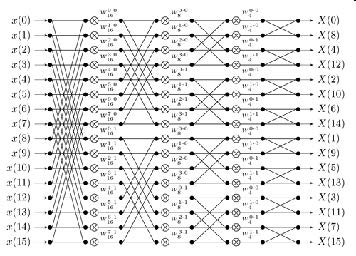
\includegraphics[width=0.7\textwidth]{spectral-methods}
    \caption{Spectral Method}
\end{figure}

\subsection{N-body methods}
Interactions between discrete points, not necessarily short-ranged i.e. Gravitational N-body

\paragraph{In general} $ O(N^2)/O(N) $
Optimizations/approximations possible are: 
\begin{itemize}
    \item Mean-field (Barnes-Hut, fast multipole, particle-in-cell) $ \implies O(N log N)/O(N) $
    or even $ O(N)/O(N) $
    \item Short-range interactions: $ \implies O(N)/O(N) $
\end{itemize}

\begin{figure}[!htbp]
    \centering
    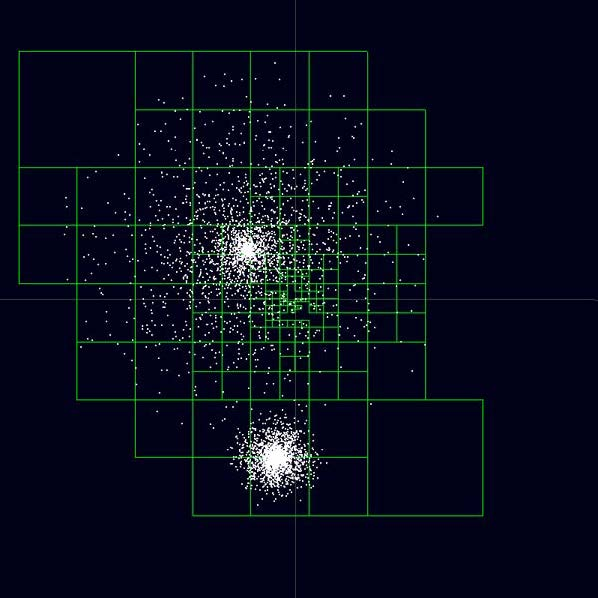
\includegraphics[width=0.7\textwidth]{n-body}
    \caption{N-body}
\end{figure}


\subsection{Structured grids}
\begin{itemize}
    \item Physical problem mapped to regular grid
    \item At the core of many PDE solvers
    \item \textbf{Simple relaxation methods:} Jacobi, Gauss-Seidel
    \item “Sweeps” are performed to update lattice sites
    \item Multigrid: Use successive grid coarsening and refinement to accelerate convergence
\end{itemize}

\begin{figure}[!htbp]
    \centering
    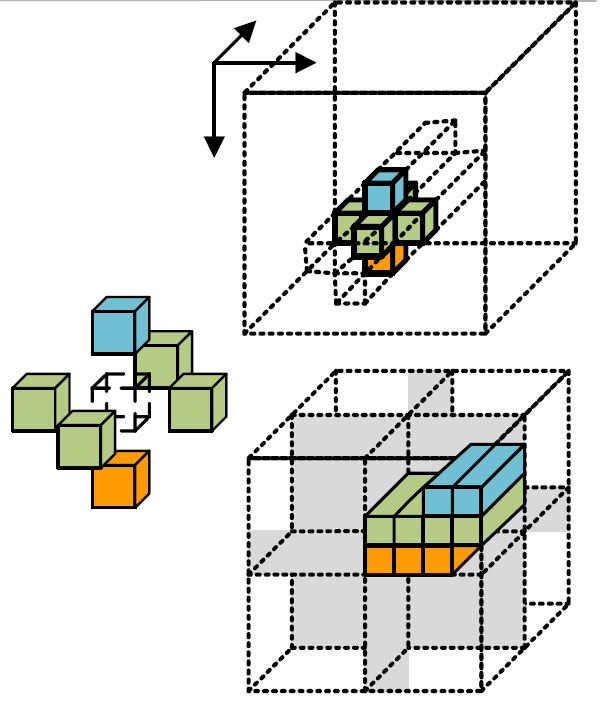
\includegraphics[width=0.7\textwidth]{structured-grids}
    \caption{Structured Grids}
\end{figure}

\subsection{Unstructured grids}
\begin{itemize}
    \item Irregular lattice, probably varying number of neighbors
    \item Neighbor relations must be explicitly stored
    \item Highly indirect data access patterns
\end{itemize}

\begin{figure}[!htbp]
    \centering
    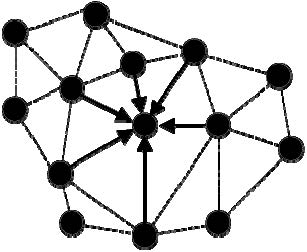
\includegraphics[width=0.7\textwidth]{unstructured-grids}
    \caption{Unstructured Grids}
\end{figure}

\subsection{Monte Carlo methods}
\begin{itemize}
    \item Computations by statistical sampling
    \item often used to cover “integration space” which would otherwise be too large to scan by brute force
    \item embarrassingly parallel
    \item Random number generation may be a bottleneck
\end{itemize}


\begin{figure}[!htbp]
    \centering
    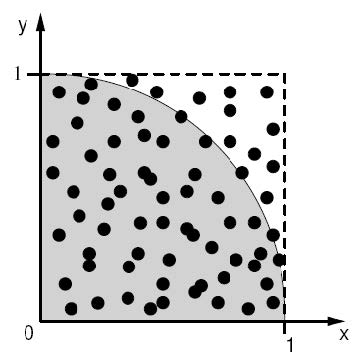
\includegraphics[width=0.7\textwidth]{monte-carlo}
    \caption{Monte Carlo methods}
\end{figure}


\section{Algorithm to solve $ n $ linear equation using pipeling}
\begin{figure}[!htbp]
    \centering
    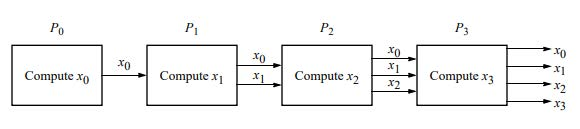
\includegraphics[width=\textwidth]{pipeline-linear-equation}
\end{figure}

\subsection{Sequential Implementation}
\begin{minted}{c}
// Seperate computation of X[0]
X[0] = B[0]/A[0][0]; 
for (int i = 1; i < n; i++) { // job for remaining ones
    int sum = 0;
    for (int j = 0; j < i; j++) {
        sum += A[i][j]*X[j];
    }
    X[i] = (B[i] - sum)/A[i][i];
}
\end{minted}

\subsection{Parallel Implementation}
\begin{minted}{c}
for (int i = 0; i < n -1; i++) {
    for (int j = 0; j < i; j++) { 
        recv(&X[j], P[i-1]);
        send(&X[j], P[i+1]);
    }
    int sum = 0;
    for (int j = 0; j < i; j++) {
        sum += A[i][j]*X[j];
    }
    X[i] = (B[i] - sum)/A[i][i];
    send(&X[i], Pi+1);
}
\end{minted}
\section{Applications for Distributed Parallel Systems}
\begin{itemize}
    \item Internet
    \item Intranet and peer-to-peer networks
    \item Email systems
    \item Cloud file backup/storage systems
    \item Electronic banking
    \item Travel reservation systems
    \item Distributed supercomputers
    \item Cloud/grid computing
    \item Mining Pool for Cryptocurrency
\end{itemize}
\section{Network Operating System Vs Distributed Operating System}
\begin{table}[H]
    \renewcommand\arraystretch{1.1}
    \hspace{-2cm}
    \begin{tabular}{p{3cm}|p{7cm}|p{7cm}}
         \textbf{Parameter} & \textbf{Network Operating System} & \textbf{Distributed Operating System} 
         \\ \hline \hline
         Definition
         & The network operating system is the platform to run a system software on a server and allow the server to manage the users, data, groups, security, applications and other networking functions. It is considered as the primary form of an operating system for the distributed architecture. The idea behind the network operating system is to permit resource sharing among two or more computers operating under their own OSs.
         & The distributed operating system handles a group of independent computers and makes them look like an ordinary centralised operating system. This is achieved by enabling the proper communication between the different computers connected with each other. The main aim of the distributed operating system is the transparency where the use of multiple hardware resources is hidden from the users. The distributed operating system is less autonomous than network operating system as the system has complete control in this environment.
         \\ \hline
         Objective 
         & Provision of local services to the remote client.
         & Management of hardware resource.
         \\ \hline
         Use 
         & Loosely coupled system employed in heterogeneous computers.
         & Tightly coupled system used in multiprocessor and homogeneous computers.
         \\ \hline
         Architecture 
         & 2-tier client/server architecture.
         & N-tier client/server architecture.
         \\ \hline
         Level of transparency  
         & Low
         & High
         \\ \hline
         Basis for communication 
         & Files
         & Shared memory and messages
         \\ \hline
         Resource Management 
         & Handled at each node.
         & Global central or distributed management.
         \\ \hline
         Implementation Complexity
         & Easy
         & Hard
         \\ \hline
         Scalability 
         & High
         & Less/moderate
         \\ \hline
         Openness 
         & Open
         & Closed
         \\ \hline
         Operating system on all nodes 
         & Can be different
         & Same
         \\ \hline
         Rate of autonomy  
         & High
         & Low
         \\ \hline
         Fault tolerance
         & Less
         & High
         \\ \hline
    \end{tabular}
    \caption{Network Operating System Vs Distributed Operating System}
    \label{tab:NetworkOSvsDistributedOS}
\end{table}

% \begin{figure}[H]
%     \centering
%     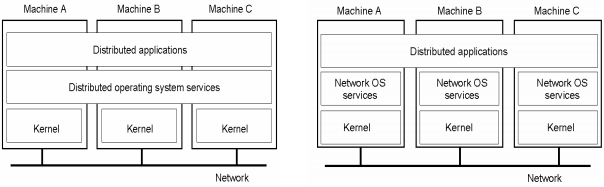
\includegraphics[width=\textwidth]{assets/distributed-operating-system}
%     \caption{Basic architecture of Distributed Operating System and Network Operating System}
%     \label{fig:NetworkOSvsDistributedOS}
% \end{figure}
\section{Transperency in Distributed Parallel Systems}
 A transparency is some aspect of the distributed system that is hidden from the user (programmer, system developer, user or application program). A transparency is provided by including some set of mechanisms in the distributed system at a layer below the interface where the transparency is required. A number of basic transparencies have been defined for a distributed system. It is important to realize that not all of these are appropriate for every system, or are available at the same level of interface. In fact, all transparencies have an associated cost, and it is extremely important for the distributed system implementer to be aware of this. Much of the text of this book describes engineering solutions to archiving these transparencies, and attempts to outline the cost of the solutions. It is a matter for much research how the costs of implementing multiple transparencies interact. This is part of current research in how to reduce operating system and communications stack overheads through such approaches as Application Layer Framing and Integrated Layer Processing. The transparencies are: 
 \begin{itemize}
     \item  \textbf{Access Transparency} There should be no apparent difference between local and remote access methods. In other words, explicit communication may be hidden. For instance, from a user's point of view, access to a remote service such as a printer should be identical with access to a local printer. From a programmers point of view, the access method to a remote object may be identical to access a local object of the same class. This transparency has two parts: 
     \begin{itemize}
         \item  Keeping a syntactical or mechanical consistency between distributed and non-distributed access, \item  Keeping the same semantics. Because the semantics of remote access are more complex, particularly failure modes, this means the local access should be a subset. Remote access will not always look like local access in that certain facilities may not be reasonable to support (for example, global exhaustive searching of a distributed system for a single object may be unreasonable in terms of network traffic). 
     \end{itemize}
     \item  \textbf{Location Transparency} The details of the topology of the system should be of no concern to the user. The location of an object in the system may not be visible to the user or programmer. This differs from access transparency in that both the naming and access methods may be the same. Names may give no hint as to location. 
     \item  \textbf{Concurrency Transparency} Users and Applications should be able to access shared data or objects without interference between each other. This requires very complex mechanisms in a distributed system, since there exists true concurrency rather than the simulated concurrency of a central system. For example, a distributed printing service must provide the same atomic access per file as a central system so that printout is not randomly interleaved. 
     \item  \textbf{Replication Transparency} If the system provides replication (for availability or performance reasons) it should not concern the user. As for all transparencies, we include the applications programmer as a user. 
     \item  \textbf{Fault Transparency} If software or hardware failures occur, these should be hidden from the user. This can be difficult to provide in a distributed system, since partial failure of the communications subsystem is possible, and this may not be reported. As far as possible, fault transparency will be provided by mechanisms that relate to access transparency. However, when the faults are inherent in the distributed nature of the system, then access transparency may not be maintained. The mechanisms that allow a system to hide faults may result in changes to access mechanisms (e.g. access to reliable objects may be different from access to simple objects). In a software system, especially a networked one, it Is often hard to tell the difference between a failed and a slow running process or processor. This distinction is hidden or made visible here. 
     \item  \textbf{Migration Transparency} If objects (processes or data) migrate (to provide better performance, or reliability, or to hide differences between hosts), this should be hidden from the user. 
     \item  \textbf{Performance Transparency} The configuration of the system should not be apparent to the user in terms of performance. This may require complex resource management mechanisms. It may not be possible at all in cases where resources are only accessible via low performance networks. 
     \item  \textbf{Scaling Transparency} A system should be able to grow without affecting application algorithms. Graceful growth and evolution is an important requirement for most enterprises. A system should also be capable of scaling down to small environments where required, and be space and/or time efficient as required. 
 \end{itemize}
\section{Application of Amdahl's law and Gustafson's law}

\subsection*{Amdahl's law}
\subsubsection*{Multiprocessing}
The original formulation of Amdahl's law states the impact of inherently sequential portion of a task on the speedup during multiprocessing. Suppose f represents the fraction of the task that is inherently sequential then using N processors the speedup is given by

\begin{equation}
    S = \frac{1}{f + (1-f) N}
\end{equation}

\[
S =
\begin{cases}
N , & \text{when } f=0; \text{resulting in an ideal linear speedup} \\
<5, & \text{when } f=0.2; \text{independent of N} \\
<2, & \text{when } f=0.5; \text{independent of N} \\
\frac{1}{f}, & \text{for large } N; \text{independent of N}
\end{cases}
\]

This relationship generates pessimism regarding the viability of massively parallel processing especially if we overestimate the value of the fraction f. But, researchers in parallel computation community started suspecting the usefulness and validity of Amdahl's law after observing impressive linear speedups in some large applications.

\subsubsection*{MEMORY HIERARCHY DESIGN}

\subsubsection*{INSTRUCTION SET AND PROCESSOR DESIGN}

\subsection*{Gustafson's law}
\begin{itemize}
    \item beam stress analysis
    \item surface wave simulation 
    \item unstable fluid flow
\end{itemize}
\section{Write  sample MPI code of work pool. Copy code and replace code fragment applying different termination approach. Briefly describe it.}
\inputminted{c}{src/workpool.c}

\subsection*{Output}
\inputminted[firstline=0,lastline=50]{text}{src/output_workpool.txt}
$\vdots$
\inputminted[firstline=900,lastline=1010]{text}{src/output_workpool.txt}

% \inputminted[firstline=0,lastline=3]{text}{src/output_ring.txt}

\end{document}
